../cictikz/src/cictikz/data/tex/cictikz_preamble.tex

% Drain current against gate voltage, on a log current axis.
%
% The straight part at low VGS is weak inversion, where the current is
% exponential in gate voltage; the bend is where the channel stops being a
% barrier problem and starts being a resistance problem. A log axis is the
% only way to see both regions in one plot, and both regions matter.
%
% Generated by py/tikzplot.py. Edit the script in ex/ that
% produced it and re-run that, not this file.

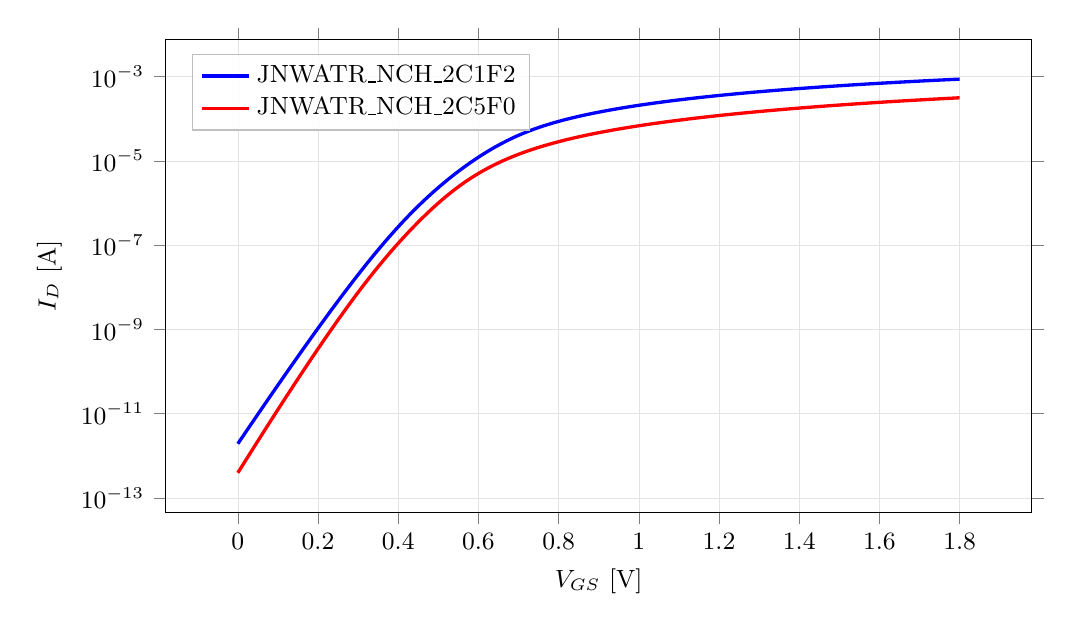
\begin{tikzpicture}[thick]

\begin{axis}[
  width=11.0cm,
  height=6.0cm,
  scale only axis,
  grid=both,
  grid style={gray!22, very thin},
  tick align=outside,
  tick label style={font=\small},
  label style={font=\small},
  title style={font=\small, yshift=-1mm},
  legend cell align=left,
  legend style={font=\small, draw=gray!50, fill=white, fill opacity=0.85, text opacity=1},
  ymode=log,
  xlabel={$V_{GS}$ [V]},
  ylabel={$I_D$ [A]},
  legend pos=north west
]
\addplot[blue, very thick, mark=none] coordinates {(0,1.9336e-12) (0.01,2.6771e-12) (0.02,3.6997e-12) (0.03,5.1092e-12) (0.04,7.0503e-12) (0.05,9.7214e-12) (0.06,1.3393e-11) (0.07,1.8437e-11) (0.08,2.5358e-11) (0.09,3.4844e-11) (0.1,4.7834e-11) (0.11,6.56e-11) (0.12,8.9872e-11) (0.13,1.2299e-10) (0.14,1.6811e-10) (0.15,2.2952e-10) (0.16,3.1295e-10) (0.17,4.2614e-10) (0.18,5.7944e-10) (0.19,7.867e-10) (0.2,1.0664e-09) (0.21,1.4431e-09) (0.22,1.9495e-09) (0.23,2.6284e-09) (0.24,3.5368e-09) (0.25,4.7489e-09) (0.26,6.3618e-09) (0.27,8.5021e-09) (0.28,1.1333e-08) (0.29,1.5066e-08) (0.3,1.9969e-08) (0.31,2.6387e-08) (0.32,3.4753e-08) (0.33,4.5614e-08) (0.34,5.9648e-08) (0.35,7.7699e-08) (0.36,1.008e-07) (0.37,1.3021e-07) (0.38,1.6746e-07) (0.39,2.1437e-07) (0.4,2.731e-07) (0.41,3.4621e-07) (0.42,4.3668e-07) (0.43,5.4799e-07) (0.44,6.8412e-07) (0.45,8.4964e-07) (0.46,1.0498e-06) (0.47,1.2904e-06) (0.48,1.5781e-06) (0.49,1.9204e-06) (0.5,2.3254e-06) (0.51,2.8024e-06) (0.52,3.3614e-06) (0.53,4.0132e-06) (0.54,4.7696e-06) (0.55,5.6431e-06) (0.56,6.6465e-06) (0.57,7.7934e-06) (0.58,9.0973e-06) (0.59,1.0571e-05) (0.6,1.2228e-05) (0.61,1.4079e-05) (0.62,1.6135e-05) (0.63,1.8404e-05) (0.64,2.0892e-05) (0.65,2.3603e-05) (0.66,2.6536e-05) (0.67,2.9691e-05) (0.68,3.3062e-05) (0.69,3.6641e-05) (0.7,4.0418e-05) (0.71,4.4382e-05) (0.72,4.8521e-05) (0.73,5.2821e-05) (0.74,5.7272e-05) (0.75,6.186e-05) (0.76,6.6577e-05) (0.77,7.1415e-05) (0.78,7.6366e-05) (0.79,8.1425e-05) (0.8,8.6586e-05) (0.81,9.1848e-05) (0.82,9.7209e-05) (0.83,0.00010267) (0.84,0.00010822) (0.85,0.00011386) (0.86,0.0001196) (0.87,0.00012543) (0.88,0.00013134) (0.89,0.00013734) (0.9,0.00014342) (0.91,0.00014959) (0.92,0.00015583) (0.93,0.00016216) (0.94,0.00016856) (0.95,0.00017503) (0.96,0.00018158) (0.97,0.00018821) (0.98,0.0001949) (0.99,0.00020166) (1,0.00020849) (1.01,0.00021538) (1.02,0.00022233) (1.03,0.00022935) (1.04,0.00023643) (1.05,0.00024357) (1.06,0.00025076) (1.07,0.00025802) (1.08,0.00026532) (1.09,0.00027269) (1.1,0.0002801) (1.11,0.00028756) (1.12,0.00029508) (1.13,0.00030264) (1.14,0.00031025) (1.15,0.0003179) (1.16,0.0003256) (1.17,0.00033335) (1.18,0.00034113) (1.19,0.00034896) (1.2,0.00035683) (1.21,0.00036474) (1.22,0.00037268) (1.23,0.00038067) (1.24,0.00038868) (1.25,0.00039674) (1.26,0.00040483) (1.27,0.00041295) (1.28,0.0004211) (1.29,0.00042928) (1.3,0.0004375) (1.31,0.00044574) (1.32,0.00045401) (1.33,0.00046231) (1.34,0.00047064) (1.35,0.00047899) (1.36,0.00048737) (1.37,0.00049577) (1.38,0.0005042) (1.39,0.00051265) (1.4,0.00052112) (1.41,0.00052961) (1.42,0.00053813) (1.43,0.00054666) (1.44,0.00055521) (1.45,0.00056378) (1.46,0.00057237) (1.47,0.00058098) (1.48,0.0005896) (1.49,0.00059824) (1.5,0.00060689) (1.51,0.00061556) (1.52,0.00062425) (1.53,0.00063294) (1.54,0.00064165) (1.55,0.00065038) (1.56,0.00065911) (1.57,0.00066786) (1.58,0.00067661) (1.59,0.00068538) (1.6,0.00069416) (1.61,0.00070295) (1.62,0.00071175) (1.63,0.00072055) (1.64,0.00072936) (1.65,0.00073819) (1.66,0.00074701) (1.67,0.00075585) (1.68,0.00076469) (1.69,0.00077354) (1.7,0.00078239) (1.71,0.00079125) (1.72,0.00080012) (1.73,0.00080898) (1.74,0.00081786) (1.75,0.00082673) (1.76,0.00083561) (1.77,0.0008445) (1.78,0.00085338) (1.79,0.00086227) (1.8,0.00087116)};
\addlegendentry{JNWATR\_NCH\_2C1F2}
\addplot[red, very thick, mark=none] coordinates {(0,3.9571e-13) (0.01,5.6151e-13) (0.02,7.9625e-13) (0.03,1.1281e-12) (0.04,1.5967e-12) (0.05,2.2578e-12) (0.06,3.1906e-12) (0.07,4.502e-12) (0.08,6.3452e-12) (0.09,8.932e-12) (0.1,1.2558e-11) (0.11,1.7632e-11) (0.12,2.4722e-11) (0.13,3.4612e-11) (0.14,4.8383e-11) (0.15,6.7524e-11) (0.16,9.4076e-11) (0.17,1.3083e-10) (0.18,1.8159e-10) (0.19,2.5154e-10) (0.2,3.4768e-10) (0.21,4.7946e-10) (0.22,6.5958e-10) (0.23,9.0502e-10) (0.24,1.2384e-09) (0.25,1.6896e-09) (0.26,2.298e-09) (0.27,3.1153e-09) (0.28,4.2085e-09) (0.29,5.6644e-09) (0.3,7.5941e-09) (0.31,1.014e-08) (0.32,1.348e-08) (0.33,1.7842e-08) (0.34,2.35e-08) (0.35,3.0812e-08) (0.36,4.0204e-08) (0.37,5.2203e-08) (0.38,6.745e-08) (0.39,8.6724e-08) (0.4,1.1096e-07) (0.41,1.413e-07) (0.42,1.7906e-07) (0.43,2.2586e-07) (0.44,2.8354e-07) (0.45,3.5425e-07) (0.46,4.4046e-07) (0.47,5.4489e-07) (0.48,6.7059e-07) (0.49,8.2079e-07) (0.5,9.9893e-07) (0.51,1.2085e-06) (0.52,1.4532e-06) (0.53,1.7363e-06) (0.54,2.0611e-06) (0.55,2.4308e-06) (0.56,2.8481e-06) (0.57,3.3153e-06) (0.58,3.8345e-06) (0.59,4.4071e-06) (0.6,5.0344e-06) (0.61,5.717e-06) (0.62,6.4555e-06) (0.63,7.2499e-06) (0.64,8.0999e-06) (0.65,9.0052e-06) (0.66,9.9651e-06) (0.67,1.0979e-05) (0.68,1.2045e-05) (0.69,1.3164e-05) (0.7,1.4333e-05) (0.71,1.5552e-05) (0.72,1.6819e-05) (0.73,1.8134e-05) (0.74,1.9495e-05) (0.75,2.09e-05) (0.76,2.235e-05) (0.77,2.3842e-05) (0.78,2.5376e-05) (0.79,2.6951e-05) (0.8,2.8566e-05) (0.81,3.0219e-05) (0.82,3.1911e-05) (0.83,3.364e-05) (0.84,3.5405e-05) (0.85,3.7206e-05) (0.86,3.9042e-05) (0.87,4.0912e-05) (0.88,4.2816e-05) (0.89,4.4754e-05) (0.9,4.6724e-05) (0.91,4.8727e-05) (0.92,5.0762e-05) (0.93,5.2828e-05) (0.94,5.4926e-05) (0.95,5.7054e-05) (0.96,5.9213e-05) (0.97,6.1401e-05) (0.98,6.362e-05) (0.99,6.5868e-05) (1,6.8145e-05) (1.01,7.0451e-05) (1.02,7.2786e-05) (1.03,7.5148e-05) (1.04,7.7539e-05) (1.05,7.9957e-05) (1.06,8.2402e-05) (1.07,8.4874e-05) (1.08,8.7373e-05) (1.09,8.9898e-05) (1.1,9.2449e-05) (1.11,9.5025e-05) (1.12,9.7626e-05) (1.13,0.00010025) (1.14,0.0001029) (1.15,0.00010558) (1.16,0.00010828) (1.17,0.000111) (1.18,0.00011374) (1.19,0.00011651) (1.2,0.0001193) (1.21,0.00012211) (1.22,0.00012495) (1.23,0.0001278) (1.24,0.00013068) (1.25,0.00013358) (1.26,0.00013649) (1.27,0.00013943) (1.28,0.00014239) (1.29,0.00014536) (1.3,0.00014836) (1.31,0.00015137) (1.32,0.0001544) (1.33,0.00015745) (1.34,0.00016051) (1.35,0.0001636) (1.36,0.00016669) (1.37,0.00016981) (1.38,0.00017294) (1.39,0.00017609) (1.4,0.00017925) (1.41,0.00018243) (1.42,0.00018562) (1.43,0.00018882) (1.44,0.00019204) (1.45,0.00019528) (1.46,0.00019852) (1.47,0.00020178) (1.48,0.00020505) (1.49,0.00020833) (1.5,0.00021163) (1.51,0.00021494) (1.52,0.00021825) (1.53,0.00022158) (1.54,0.00022492) (1.55,0.00022827) (1.56,0.00023163) (1.57,0.000235) (1.58,0.00023838) (1.59,0.00024177) (1.6,0.00024517) (1.61,0.00024857) (1.62,0.00025199) (1.63,0.00025541) (1.64,0.00025884) (1.65,0.00026228) (1.66,0.00026572) (1.67,0.00026918) (1.68,0.00027263) (1.69,0.0002761) (1.7,0.00027957) (1.71,0.00028305) (1.72,0.00028653) (1.73,0.00029002) (1.74,0.00029351) (1.75,0.00029701) (1.76,0.00030051) (1.77,0.00030402) (1.78,0.00030753) (1.79,0.00031105) (1.8,0.00031457)};
\addlegendentry{JNWATR\_NCH\_2C5F0}
\end{axis}

\end{tikzpicture}
\end{document}
